\documentclass[tikz,border=12pt]{standalone}
\usepackage{amsmath,amssymb}
\usetikzlibrary{calc,arrows.meta,decorations.markings}

\tikzset{
  midarrow/.style={decoration={markings, mark=at position 0.55 with {\arrow{Stealth[length=6pt]}}}, postaction={decorate}},
  midarrow2/.style={decoration={markings, mark=at position 0.65 with {\arrow{Stealth[length=6pt]Stealth[length=6pt]}}}, postaction={decorate}}
}

\begin{document}
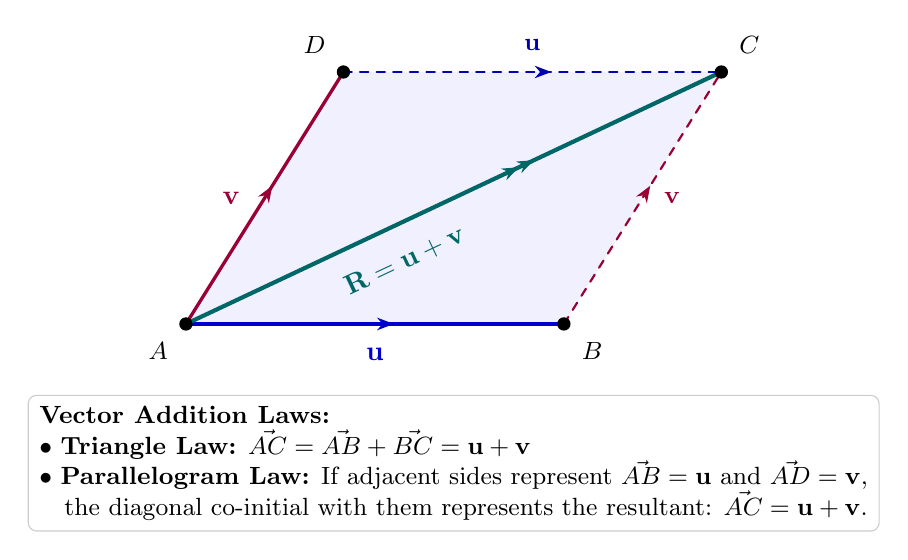
\begin{tikzpicture}[>=latex, line cap=round, line join=round]

  % Coordinates of the Parallelogram of Vectors
  \coordinate (A) at (0, 0);
  \coordinate (B) at (4.8, 0);
  \coordinate (D) at (2.0, 3.2);
  \coordinate (C) at (6.8, 3.2);

  % Shading of the parallelogram
  \fill[blue!6] (A) -- (B) -- (C) -- (D) -- cycle;

  % Parallelogram completion lines (dashed with midway arrows)
  \draw[thick, dashed, purple!80!black, midarrow] (B) -- (C) node[midway, right=4pt, font=\small\bfseries] {$\mathbf{v}$};
  \draw[thick, dashed, blue!70!black, midarrow] (D) -- (C) node[midway, above=4pt, font=\small\bfseries] {$\mathbf{u}$};

  % Primary vectors u and v from origin A (with midway arrows)
  \draw[very thick, blue!80!black, midarrow] (A) -- (B) node[midway, below=5pt, font=\normalsize\bfseries] {$\mathbf{u}$};
  \draw[very thick, purple!80!black, midarrow] (A) -- (D) node[midway, left=5pt, font=\normalsize\bfseries] {$\mathbf{v}$};

  % Resultant diagonal vector R = u + v with double arrowhead midway and sloped label
  \draw[line width=1.5pt, teal!80!black, midarrow2] (A) -- (C) node[pos=0.38, sloped, below=5pt, font=\normalsize\bfseries, teal!80!black] {$\mathbf{R} = \mathbf{u} + \mathbf{v}$};

  % Vertex points
  \filldraw[black] (A) circle (2.2pt) node[below left=3pt, font=\small\bfseries] {$A$};
  \filldraw[black] (B) circle (2.2pt) node[below right=3pt, font=\small\bfseries] {$B$};
  \filldraw[black] (C) circle (2.2pt) node[above right=3pt, font=\small\bfseries] {$C$};
  \filldraw[black] (D) circle (2.2pt) node[above left=3pt, font=\small\bfseries] {$D$};

  % Explanatory Card / Annotation below
  \node[align=left, font=\small, fill=white, inner sep=4pt, draw=gray!40, rounded corners=3pt, anchor=north] at (3.4, -0.9) {
    \textbf{Vector Addition Laws:}\\
    $\bullet$ \textbf{Triangle Law:} $\vec{AC} = \vec{AB} + \vec{BC} = \mathbf{u} + \mathbf{v}$\\
    $\bullet$ \textbf{Parallelogram Law:} If adjacent sides represent $\vec{AB} = \mathbf{u}$ and $\vec{AD} = \mathbf{v}$,\\
    \hspace*{3.2mm}the diagonal co-initial with them represents the resultant: $\vec{AC} = \mathbf{u} + \mathbf{v}$.
  };

\end{tikzpicture}
\end{document}
